\documentclass[journal=jacsat,manuscript=article,layout=twocolumn]{achemso}
%   \usepackage[version=3]{mhchem} % Formula subscripts using \ce{}
\usepackage[T1]{fontenc}       % Use modern font encodings
% \usepackage[active]{preview}
%EXTRA PACKAGES%
% \usepackage{multicol}
\usepackage{xcolor}
\usepackage{textcomp}
\usepackage{geometry}
\usepackage[normalem]{ulem}
\usepackage{amsmath}

%%%%%%%%%%%%%%%%%%%%%%%%%%%%%%%%%%%%%%%%%%%%%%%%%%%%%%%%%%%%%%%%%%%%%
%% Place any additional macros here.  Please use \newcommand* where
%% possible, and avoid layout-changing macros (which are not used
%% when typesetting).
%%%%%%%%%%%%%%%%%%%%%%%%%%%%%%%%%%%%%%%%%%%%%%%%%%%%%%%%%%%%%%%%%%%%%
\newcommand*{\ga}{\alpha}
\newcommand*{\gb}{\beta}
\newcommand*{\gam}{\gamma}
\newcommand*{\gd}{\delta}
\newcommand*{\eps}{\epsilon}
\newcommand*{\veps}{\varepsilon}
\newcommand*{\gz}{\zeta}
\newcommand*{\gt}{\theta}
\newcommand*{\gi}{\iota}
\newcommand*{\gk}{\kappa}
\newcommand*{\gl}{\lambda}
\newcommand*{\gs}{\sigma}
\newcommand*{\go}{\omega}
\newcommand*{\Gam}{\Gamma}
\newcommand*{\gD}{\Delta}
\newcommand*{\gT}{\Theta}
\newcommand*{\gL}{\Lambda}
\newcommand*{\gS}{\Sigma}
\newcommand*{\gO}{\Omega}
\newcommand*{\pt}[1]{\left( #1\right)}
\newcommand*{\pq}[1]{\left[ #1 \right]}
\newcommand*{\pg}[1]{\left\{ #1\right\}}
\newcommand*{\figref}[1]{\figurename~\ref{#1}}
\newcommand*{\red}[1]{\textcolor{red}{#1}}
\newcommand*{\blue}[1]{\textcolor{blue}{#1}}
\newcommand*{\gray}[1]{\textcolor{gray}{#1}}
% \renewcommand{\baselinestretch}


%%%%%%%%%%%%%%%%%%%%%%%%%%%%%%%%%%%%%%%%%%%%%%%%%%%%%%%%%%%%%%%%%%%%%
%% Meta-data block
%% ---------------
%% Each author should be given as a separate \author command.
%%
%% Corresponding authors should have an e-mail given after the author
%% name as an \email command. Phone and fax numbers can be given
%% using \phone and \fax, respectively; this information is optional.
%%
%% The affiliation of authors is given after the authors; each
%% \affiliation command applies to all preceding authors not already
%% assigned an affiliation.
%%
%% The affiliation takes an option argument for the short name.  This
%% will typically be something like "University of Somewhere".
%%
%% The \altaffiliation macro should be used for new address, etc.
%% On the other hand, \alsoaffiliation is used on a per author basis
%% when authors are associated with multiple institutions.
%%%%%%%%%%%%%%%%%%%%%%%%%%%%%%%%%%%%%%%%%%%%%%%%%%%%%%%%%%%%%%%%%%%%%
\author{Elizaveta Guseva}
\email{elizaveta.guseva@stonybrook.edu}
\affiliation[Stony Brook University]
{Laufer Center for Physical and Quantitative Biology, Stony Brook University, Stony Brook, NY, (United States)}
% \altaffiliation{A shared footnote}
\author{Ronald N Zuckermann}
\affiliation{Lawrence Berkeley National Laboratory (LBNL), Berkeley, CA (United States)}
\author{Ken A Dill}
\email{dill@laufercenter.org}
\phone{+1631 632 5400}
\fax{+1631 632 5405}
\affiliation[Stony Brook University]
{Laufer Center for Physical and Quantitative Biology, Stony Brook University, Stony Brook, NY, (United States)}


%%%%%%%%%%%%%%%%%%%%%%%%%%%%%%%%%%%%%%%%%%%%%%%%%%%%%%%%%%%%%%%%%%%%%
%% The document title should be given as usual. Some journals require
%% a running title from the author: this should be supplied as an
%% optional argument to \title.
%%%%%%%%%%%%%%%%%%%%%%%%%%%%%%%%%%%%%%%%%%%%%%%%%%%%%%%%%%%%%%%%%%%%%
\title[]
  {Prebiotic polymers: a mechanism that could produce long informational chains}

%%%%%%%%%%%%%%%%%%%%%%%%%%%%%%%%%%%%%%%%%%%%%%%%%%%%%%%%%%%%%%%%%%%%%
%% Some journals require a list of abbreviations or keywords to be
%% supplied. These should be set up here, and will be printed after
%% the title and author information, if needed.
%%%%%%%%%%%%%%%%%%%%%%%%%%%%%%%%%%%%%%%%%%%%%%%%%%%%%%%%%%%%%%%%%%%%%
\abbreviations{IR,NMR,UV}
\keywords{American Chemical Society, \LaTeX}

%%%%%%%%%%%%%%%%%%%%%%%%%%%%%%%%%%%%%%%%%%%%%%%%%%%%%%%%%%%%%%%%%%%%%
%% The manuscript does not need to include \maketitle, which is
%% executed automatically.
%%%%%%%%%%%%%%%%%%%%%%%%%%%%%%%%%%%%%%%%%%%%%%%%%%%%%%%%%%%%%%%%%%%%%



\begin{document}
\abstract{\footnotesize Many studies have found that amino acids or nucleic acids can polymerize 
under prebiotic conditions.  But, the products are mostly short random sequences.  It remains a 
puzzle to understand how long and specific sequences of proteins, DNA or RNA might have arisen 
prebiotically.  Here, we study the HP model of polymers made of hydrophobic (H) and polar (P) 
monomers.  It is known that even relatively short random HP chains will ball up into compact 
structures, often resembling folded states of proteins.  Here, we first show that folding alone does 
not provide an answer.  But we also find that folding plus primitive catalysis, mediated by 
hydrophobic interactions, can lead to the amplification of specific sequences of longer chain 
polymers from conditions that otherwise provide synthesis of short random polymers.  This could be a 
mechanism that was relevant in the early origins of life.}

%%%MAIN TEXT%%%%

 
\section{Introduction} 

We are interested in two puzzles about the early origins of life: How might prebiotic polymerization
processes have produced long chains of protein-like or nucleic-acid-like molecules?  And, how could 
random processes acting on random sequences have led to early sequence-structure 
relationships~\cite{Joyce1987,Abel2005}?

Many experiments show that either amino acids or nucleotides can polymerize into short-chain 
molecules under prebiotic conditions without the presence of enzymes
\cite{Shock1992,Martin1998,PAECHT-HOROWITZ1970,Leman2004a,Orgel2004}.  
It is also known that the yields of such short-chain oligomers can be increased under 
prebiotically plausible conditions by such processes as adsorption to 
clays\cite{Rao1980,Lambert2008} or minerals\cite{Bernal1949,Ferris1996}, by evaporation of tidal 
pools\cite{Nelson2001}, by concentration in ice through eutectic melts \cite{Kanavarioti2001} or 
freezing\cite{Bada2004} or temperature cycles. 

It remains a puzzle, however, to understand how prebiotic processes could have overcome what 
we call the ``Flory Problem'' -- the production of long-chain polymers.  It is generally assumed 
that the minimum chain lengths of proteins or nucleic acids that are needed to make the complex 
structures essential for biological function is estimated to be around 30-60 monomers long 
\cite{Szostak1993}.  Yet, since the earliest work of Flory and others, which elucidated basic 
mechanisms of chain polymerizations, it has been clear that chain syntheses are stochastic, whereby 
the concentrations of longer chains are exponentially smaller than of shorter chains. 

Correspondingly, 
\sout{it is known that}\footnote{\red{Here, we say it is known then one can get 
only short sequences, and then mention studies. It looks like people tried to prove this point with 
their studies, but they in fact tried to overcome difficulties, like no polymerization in water 
solutions at all. }} 
\textbf{experimental studies which are intended to find out possible ways of } 
prebiotic polymerizations of 
amino acids and nucleotides 
lead predominantly to short chains. Leman et al. 
showed that carbonyl sulfide (COS), a simple 
volcanic gas, brings about the formation of oligo-peptides from amino acids under mild conditions in 
aqueous solution in minutes to hours. But the product is mainly dimers and 
trimers~\cite{Leman2004a}.  In another study, using various mineral catalysts such as calcium 
montmorillonite, hectorite, silica or alumina, mixtures of Gly and Gly$_2$ grow to about 6-mers 
after 14 days~\cite{Rode1997,Rode1999}.  Or, by freezing samples of phosphoimidazolide-activated 
uridine in the presence of metal ions in dilute solutions, Kanavarioti found polymers of 
oligouridylates up to 11 bases long, with an average length of 4 \cite{Kanavarioti2001}.  And, 
starting from decanucleotides [$^{32}$P]dA(pdA)$_8$pA adsorbed on Na$^+$-montmorillonite, Ferris et 
al. observed chains averaging lengths 20-40 after 14 days at 25\textcelsius\ \cite{Ferris1996}.  It 
is not yet understood how prebiotic polymerizations could lead to the types of long protein or 
nucleic-acid chains that are found in present-day cells.



   
\section{The ``Flory problem'' of obtaining long chains}
\label{sec:flory} 
The standard stochastic processes of chain polymerization lead to the the Flory or 
Flory-Schulz distribution of the concentrations of chains of different chain 
lengths~\cite{Flory1953}. 
\begin{equation}
 f(a)=a^2l(1-a)^{l-1},
\end{equation} 
where $l$ is the chain length and $a$ is the probability of chain termination, 
which is a measure of the average chain length: $\langle l \rangle = a(2- a)$.
Figure \ref{fig:flory} shows the central prediction of Flory theory, that 
longer chains are exponentially less populated than shorter chains.  For example (see the blue line 
in Fig~\ref{fig:flory}):
\begin{equation}
  \frac{\pq{10~\mathrm{mers}}}{\pq{1~\mathrm{mers}}}\propto10^{-4},\qquad\frac{\pq{20~\mathrm{mers}}}{\pq{1~\mathrm{mers}}}\propto10^{-9}
\end{equation} 
Thus, for a synthetic process that starts with micro-molar concentrations of monomers, the 
average chain length would be $\langle l \rangle = 2$ and 40-mers would have 
negligible concentrations of $\propto 10^{-19} $ mol/L. 
\begin{figure}[h!]
  \centering
  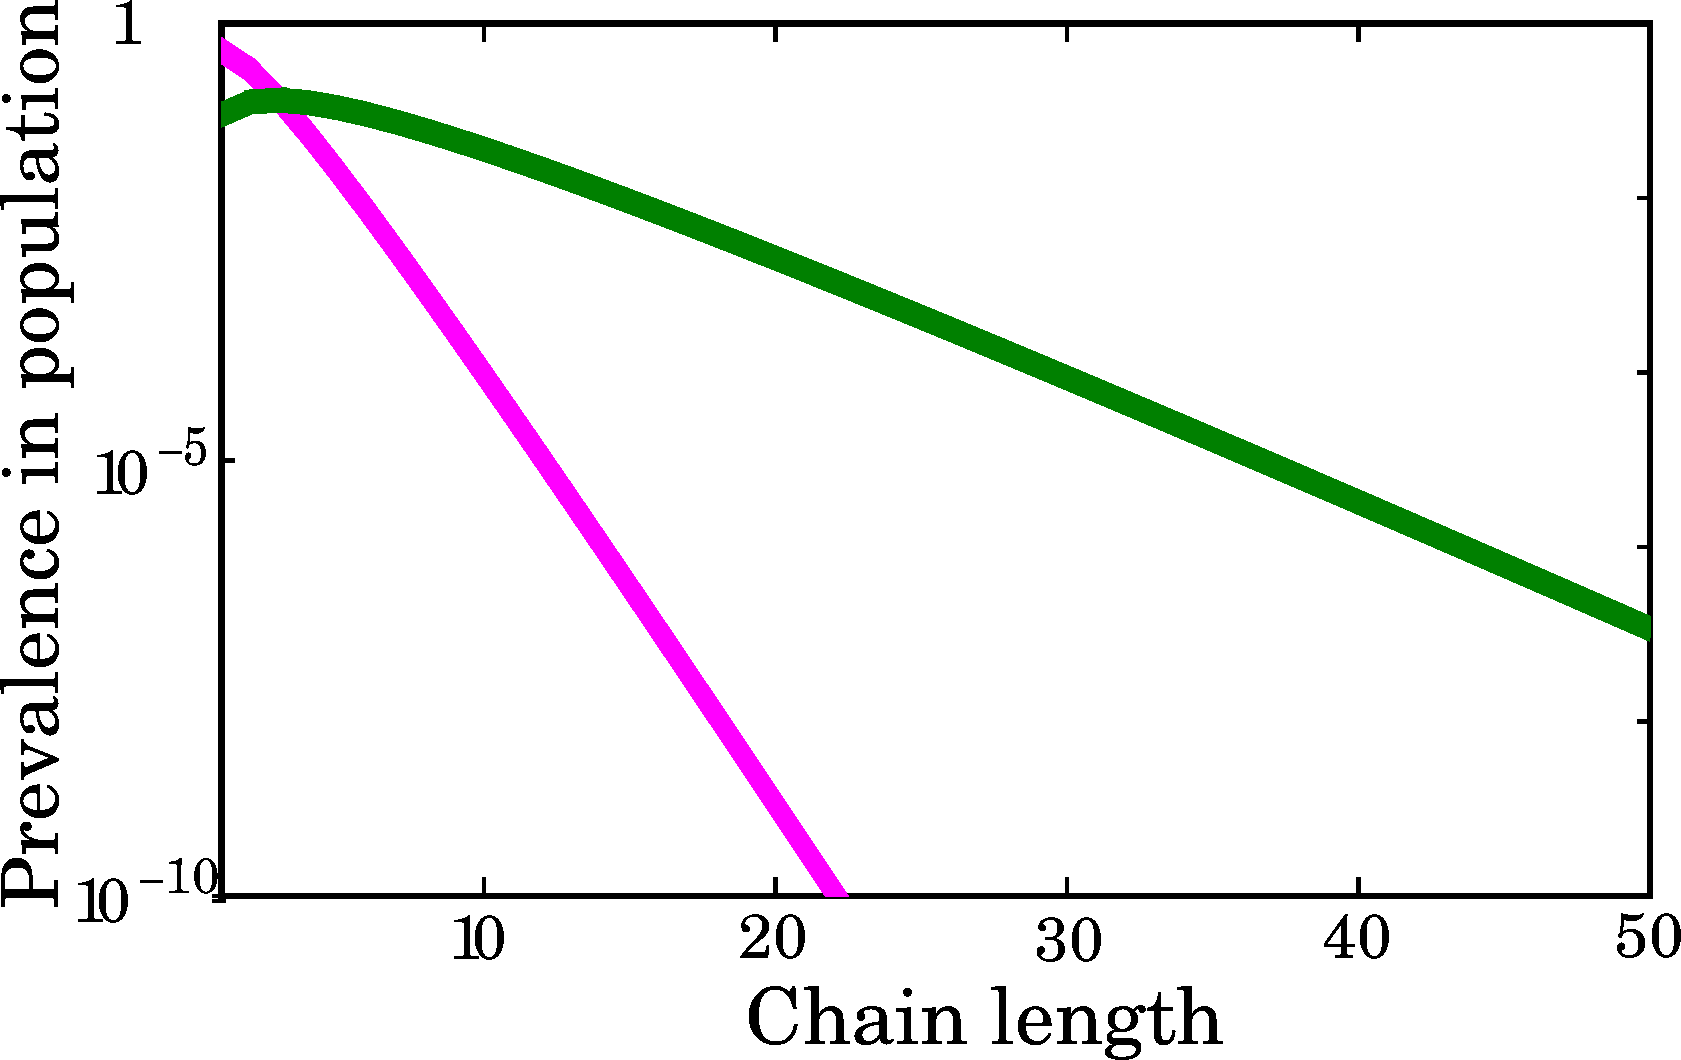
\includegraphics[width=\columnwidth]{pictures/flory2.pdf} 
  \caption{The Flory length distribution that arises from spontaneous polymerization processes.}
  \label{fig:flory}
\end{figure}

The Flory distribution is a good model of prebiotic syntheses of peptide and nucleic 
acid chains.  Figure~\ref{fig:some_flory} shows that the Flory model fits known length 
distributions from various prebiotic syntheses (sometimes data is fit to an exponential law, 
$f(a)\propto const^l$, which is slightly simpler but nearly identical in form 
~\cite{nowak2008prevolutionary,Derr2012}).  So, since prebiotic chemistry appears to give 
submillimolar or submicromolar 
concentrations\cite{Aubrey2009,Kanavarioti2001,Lazcano1996}\red{check citations} of monomers, 
longer chains have been expected to be 
present in negligible concentrations.  The Flory 
problem is not solved by improving the catalyst~\cite{Derr2012}. The problem is in the equilibrium, 
not the kinetics.  The slope of the Flory plot is governed by $a$, the equilibrium constant for 
bonding each monomer into the chain.

\begin{figure}[h!]
  \centering
  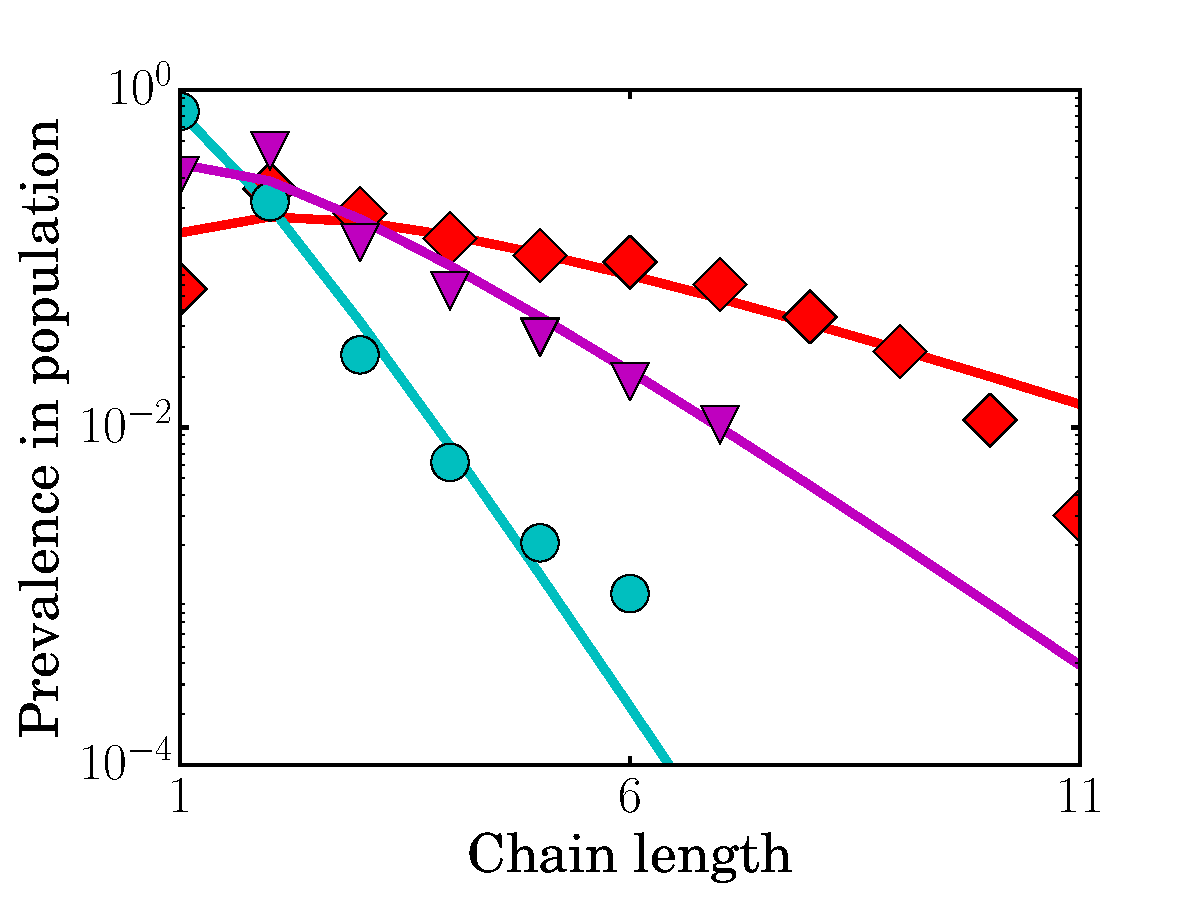
\includegraphics[width=\columnwidth]{pictures/some_flory.pdf} 
  \caption{Chain-length distributions of peptides and nucleic acids synthesized under prebiotic 
conditions.  The lines show curve fits to the Flory distribution for polymerization processes. Data 
points: red -- Kanavarioti~\cite{Kanavarioti2001}, cyan -- Ding~\cite{Ding1996}, 
magenta -- Ferris~\cite{Ferris1999}}
  \label{fig:some_flory}
\end{figure}


\section{Proposal: the key prebiotic molecules were HP polymers}

 A key premise of the present work is that some puzzles of prebiotic chemistry may be 
 resolvable by recognizing the special properties of HP polymers.  HP polymers are copolymers in 
which the monomer units can be categorized as hydrophobic (H) or polar (P)\textbf{, in particular 
sequences}\red{??}. 
 An example of present-day HP polymers is proteins: the 20 amino acids can be divided into H or P.  
In HP polymers, the sequence patterning of the H and P monomers lead to a solvation-based encoding 
of sequence-structure relationships~\cite{Chan1991}.  Our studies below lead to two main 
conclusions.  First, 
even random processes that synthesize random HP sequences will lead to some selection that can 
concentrate some sequences and structures over others.  Second, some folded HP sequences can have 
primitive catalytic and autocatalytic abilities, based on their exposed hydrophobic surfaces, 
whereby certain chains can help to polymerize other chains.  Thus, HP polymers appear to have 
features that can explain how prebiotic chemistry might escape the Flory Problem.  

HP polymers have been studied extensively as a model for the folding and 
evolution of proteins~\cite{lau1989lattice,Chan1991,Miller1995,Yue1995,agarwala1997local}.  Such 
studies have shown that stably folded structures of proteins to a large extent can be explained by 
binary pattern of polar and hydrophobic residues and do not require knowledge of specific 
interresidue contacts~\cite{Yue1992,Xiong1995,Fisher2011}. They have further demonstrated that 
a large fraction of the space of random sequences can 
collapse into compact structures resembling native proteins\cite{lau1989lattice}; see fig. 
\ref{fig:hydro-effect}.  RNA molecules are also able to fold in water, indicating differential 
solvation.  While our present model focuses on hydrophobic interactions, it is simply intended as a 
concrete model of solvation, that could more broadly include hydrogen bonding or other interactions. 
 So, our analysis below is not limited to proteins as foldamers.

\begin{figure}[h!]
  \centering
  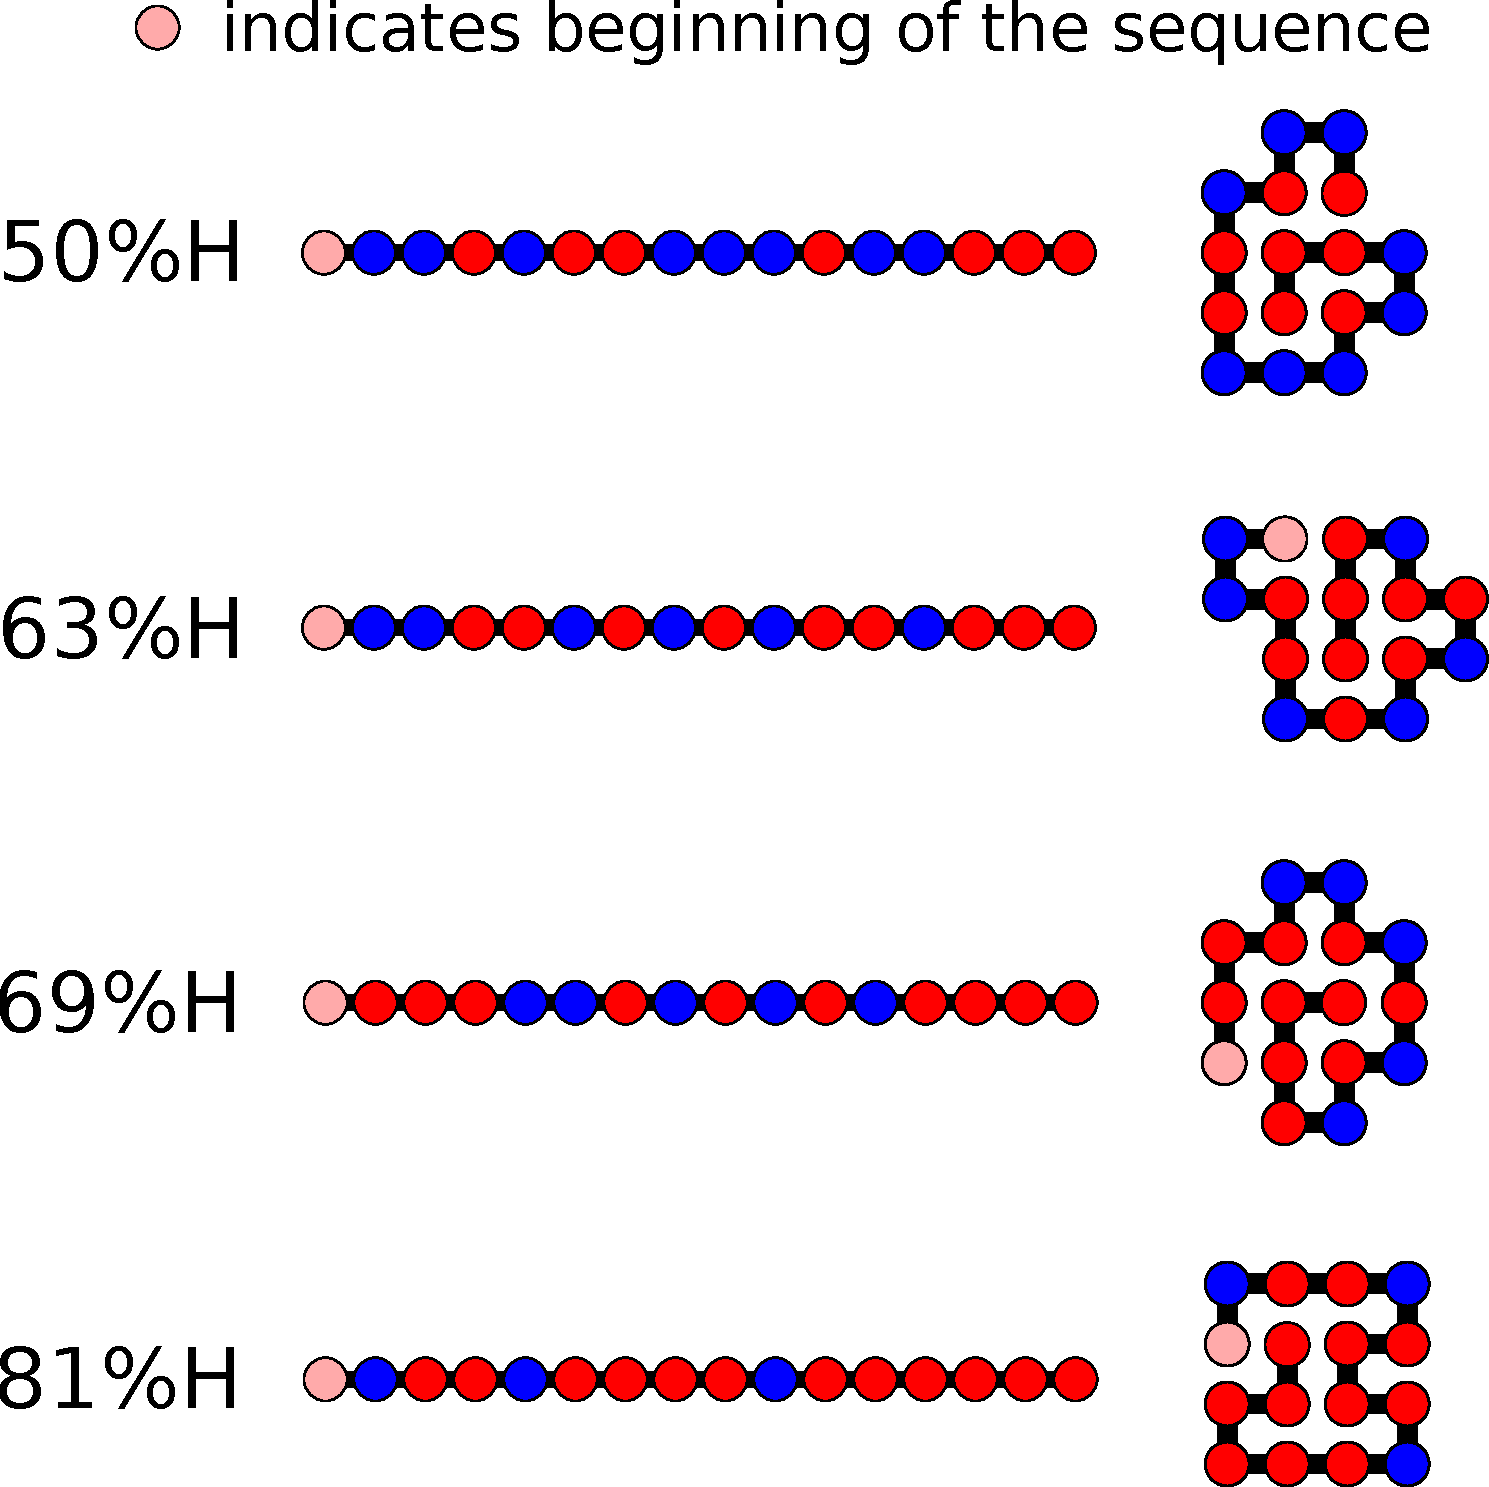
\includegraphics[width=\columnwidth]{pictures/tst-seqs.pdf} 
  \caption{HH interactions are favorable in water, leading to different 
compact states for different 
HP sequences.}
  \label{fig:hydro-effect}
\end{figure}


\section{The model for HP polymerization kinetics}

 We consider a soup containing $H$ and $P$ monomers \sout{at concentration xxx} \red{There is no 
indication of concentration in our system. I have ``populations'' and they vary largly. Maybe we 
shouldn't mention any concentrations at all}.  
 A prerequisite for prebiotic origins are processes that are away from equilibrium.  In our case, 
(``food'') monomers are supplied by 
an external source with rate $a$ and any molecule be removed from the system with rate $d$; this 
mimics cell growth and division. We assume a system in which activated monomers are plentiful\sout{, 
at concentration xxx}\red{For activated monomers populations/concentration are purely abstract 
ideas.}, and therefore any given polymer in solution elongates spontaneously with rate $\ga$.  
Without loss of generality we set the rate units of this model so that this parameter 
equals 1; all other rates are taken relative to this growth rate.  We assume all polymers also 
undergo spontaneous hydrolysis; any bond can be broken with rate constant $d_h$.

 Now, in addition to this basic polymerization dynamics, we also account 
 for the fact that some sequences will fold into native HP structures, protecting its hydrophobic 
core residues from hydrolysis.  In the standard definition for HP polymers, we regard a chain as 
folded if it has a unique lowest-energy structure.  That is, some sequences have only a single 
conformation giving a maximum number of HH noncovalent contacts.  (Most sequences, in contrast, have 
many low-energy states; we do not count these as folded structures.)  The conformational energy of 
the native fold ($E_{nat}$) of any particular folded sequence equals the number of hydrophobic 
interactions ($n_{h\phi}$) $\times$ the energy $E_H$, of one hydrophobic interaction, which is known 
to be $\approx 1-2kT$\cite{Ghosh2009}:
\begin{equation}
 E_{nat}=n_{h\phi}E_H.
\end{equation} 
This energy differs for different sequences.  Now, given knowledge of $E_{nat}$ for any particular 
sequence, we can readily compute the folding and unfolding rate coefficients from~\cite{Ghosh2009}:
\begin{equation}
 \ln\pt{\frac{k_f}{k_u}}=-\gD G/kT = E_{nat}/kT-N\ln z,
\end{equation} 
for reversible folding, where $z$ is the number of rotational degrees of freedom per peptide bond.  
For proteins in aqueous solution, the parameters are known~\cite{Ghosh2010,Dill2011} \red{(see 
appendix)}, 
giving the following expressions for folding and unfolding rates:
\begin{equation}
\begin{split}
  k_u &= \exp[16.15-1.28 \sqrt{N} -E_H(0.5 N + 1.34)],\\
  k_f &= k_u\exp(\gD G)
\end{split}
\end{equation}

\red{\textbf{Check constants with final simulation results}}

\blue{E -- We need more methods description here.  (1) We need to say how the folding and 
unfolding rates affect polymerization.  Which chains get removed from further elongation?  And, we 
need to similarly describe how aggregation adds or eliminates chains from polymerization.  We need a 
little description of how each sequence gets treated within your kinetics modeling.  Maybe give a 
descriptive example or two: a protein that doesn't fold can be hydrolyzed everywhere, a protein that 
does fold is only hydrolyzable at certain sites, a protein that folds and has a hydrophobic surface 
patch can also catalyze another chain, ...}

Catalysis rate is proportional to the exponent of hydrophobic energy $E_H$ and number of 
contacting hydrophobes $n_c$: $\ga\cdot\exp(E_{H}\cdot n_{c}/kT)$. Some experiments also include 
aggregation reactions for the long hydrophobic chains.

Here is how we perform each calculation.  Monomers enter the system with rate constant $a\gg1$.  
\blue{E - What is the rate that monomers enter? }\red{200. It's pretty random number just 
any which is big enough} \blue{Is it different than the rate that activated monomers enter?} 
\red{They don't enter}  \blue{Is there a rate that activated monomers leave?  If so, why? What's the 
physics you envision } \red{Every molecule can leave, not only monomers. It represents dilution, 
diffusion or whichever sink we can imagine.}
 



\section{HP chain folding alone does not solve the Flory Problem}
Our first computational experiment asks whether HP chain folding alone is sufficient to 
alter the Flory chain-length polymerization distribution.  In short, we ask whether the few randomly 
synthesized sequences that happen to fold, which therefore also happen to protect their interior 
residues from hydrolysis, lead to changing the Flory length distribution?  Details are in 
experiment 
2; see Simulations, compared to Simulations  Experiment 1, which has the 
hydrophobic energy set to 0 and run simulations without folding or catalysis.  
Figure~\ref{fig:sim.flory-fold} 
shows that chain folding alone, of the few foldable sequences, is not sufficient to escape the Flory 
problem of the exponentially diminishing concentrations of chains with length.  Folding does 
increase the abundances of some of the folded sequences.  But, their instances are so rare that they 
do not alter the distribution.  Thus, folding alone does not appear to explain how prebiotic 
polymers escape the Flory Problem.

\begin{figure}[h!]
  \centering
  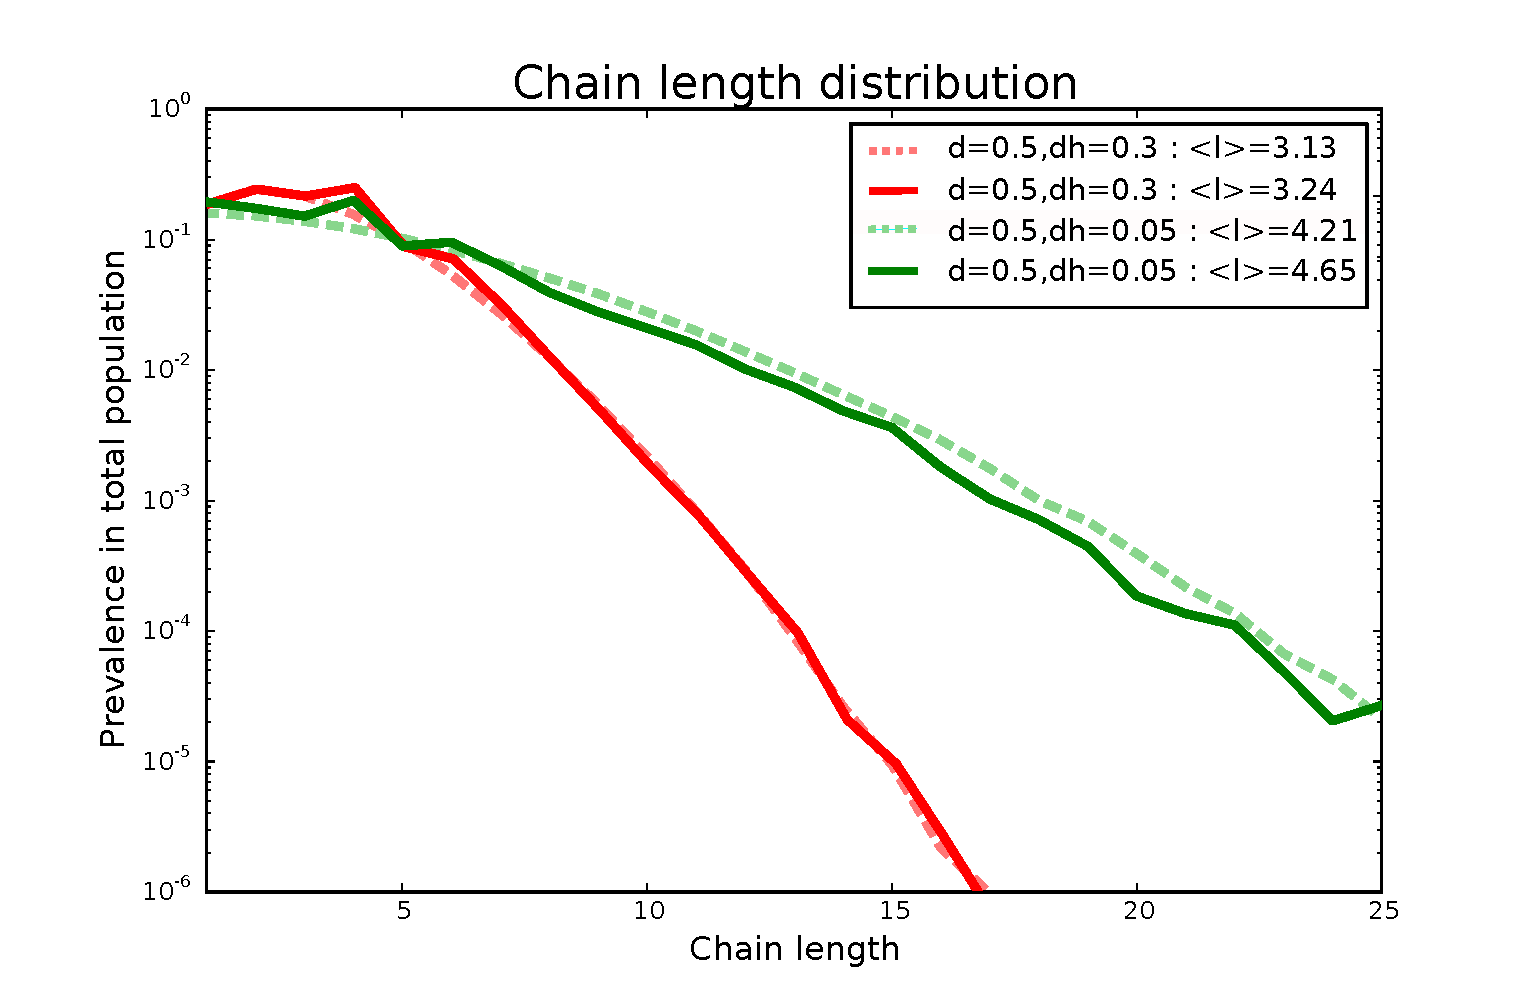
\includegraphics[width=\columnwidth]{pictures/flory-and-fold.pdf} 
  \caption{Dashed lines represent polymerization without folding or catalysis. Solid lines 
correspond to simulations run with folding but without catalysis. For details of simulations see 
section \ref{sec:mat-sim}, Experiment 2. }
  \label{fig:sim.flory-fold}
\end{figure}

\section{Some HP-foldamers can also be catalysts}

Here, we consider another property of foldamers such as proteins; namely their ability 
to catalyze reactions.   Present-day foldamers (proteins and RNA molecules) can catalyze reactions 
very efficiently -- including the reaction in the ribosome that synthesizes the peptide 
bond~\cite{Stachelhaus1998}. These modern catalysts have evolved over a long time towards 
exceptional catalytic functionalities.  Of course, prebiotic functionalities are likely to have been 
much more primitive.  Our interest here is in how the most primitive catalysts might have begun.  
Precision and complexity isn't a requirement for peptides to perform biological function. Studies 
show that folded proteins generated from random libraries can sustain the growth of living 
cells~\cite{Fisher2011} and specific bindings between them and small molecules are not 
rare~\cite{Cherny2012}. These findings imply that some primitive foldamers could have had some 
primitive catalytic capability.  The unique power in catalysis of a foldamer -- in contrast to other 
polymeric structures -- is that it can resemble a microscale solid, with very precise positioning of 
different chemical moieties over sufficiently long time scales that substrates and transition states 
can `recognize', bind, and react on them.  For example, serine proteases utilize a catalytic triad 
of 3 amino acids.  So, foldability in some type of prebiotic polymer, could conceivably have had a 
special role in allowing for primitive catalysis.  Here, we use a toy model to capture that simple 
idea, namely that a folded polymer can position a small number of residues in a way that can 
catalyze a reaction.  

Fig. \ref{fig:hp-catalysis} shows the basic idea.  Suppose a polymer molecule $A$ folds 
so that it has 
exposed hydrophobic monomers on its surface.  This patch can serve as a sticky spot for 
another HP molecule $B$ and for an H monomer $C$.  Hydrophobic interaction between three of them 
localizes growing chain and next monomer and reduces the kinetic barrier of polymerization for $B$ 
and $C$ molecules.  A typical hydrophobic 
interaction is $1-2kT$.  Consequently chain $A$ is a catalyst that provides a hydrophobic 
landing pad and reduces activation energy by 3-4 hydrophobic interactions, thereby increasing the 
polymerization rate around $ 100$-fold (fig.~\ref{fig:hp-catalysis-b}).  Of course, this rate 
enhancement is much smaller than the $10^7$-fold of modern 
ribosomes~\cite{Sievers2004a}. Nevertheless, it gives a conceptual basis for how peptide-bond 
formation rate enhancements might have had their prebiotic beginnings.


Before proceeding further, we note what is intended in our model and what is not.  It is is not 
supposed to be an accurate depiction of any real catalytic mechanism.  Rather, it is a toy 
model of a possible mechanism.  In this case, the mechanism is simply translational 
localization of the two reactants, polymer $B$ and monomer $C$ for extending the chain.  At the 
present time, this coarse-grained simplification is the only unbiased and practical type of model 
that can estimate the size of protein sequence space relevant for such catalysis.
\begin{figure}[h!]
  \centering
  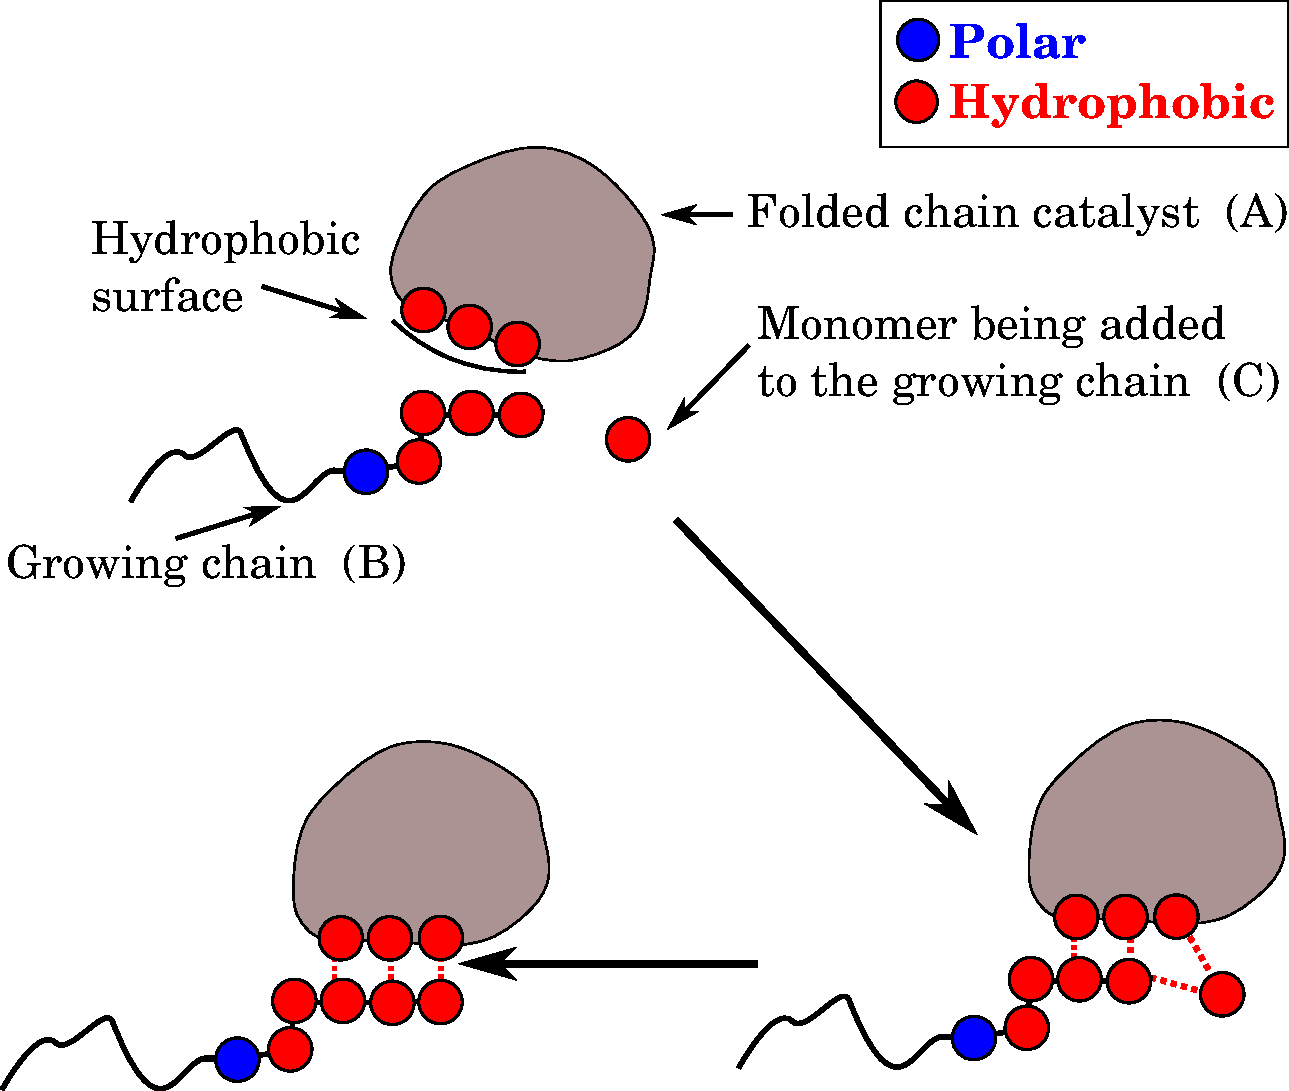
\includegraphics[width=0.9\columnwidth]{pictures/hp-catalysis.pdf} 
  \caption{Chain $A$ folds so that it has exposed hydrophobic monomers on its surface.  This patch 
can serve as a sticky spot for another HP molecule $B$ and for an H monomer $C$.  Hydrophobic 
interaction between three of them localizes growing chain and next monomer and reduces the kinetic 
barrier of polymerization for $B$ and $C$ molecules by 3-4 hydrophobic interactions, increasing the 
polymerization rate around $ 100$-fold }
  \label{fig:hp-catalysis}
\end{figure}


\subsection{HP foldamer-catalysts can solve the Flory Problem}

Figure~\ref{fig:sim.flory-fold} shows the results of simulations, now allowing for both the 
folding of all HP sequences, according to the rules of the HP model, and allowing for catalysis 
based on all those foldamers that have three $H$ monomers on their surfaces in their unique native 
folded states (see SI for details). Presence of catalysis in the system skews the distribution 
significantly. This distribution is fairly stable towards hydrolysis and dilution
parameters. It allows for 1 order of magnitude change in those parameters without significant change 
in the behavior of the system. Sequences responsible for the skew of the distribution are few 
in numbers they all are catalysts and have long stretches of hydrophobes, which also means that they 
are products of catalysis. 

This figure makes a key point of this paper, namely that the catalysis that results from some 
foldamers -- even though it is weak -- can lead to solving the Flory Problem. \red{This claim isn't 
true in general. There are plenty of systems with catalysis, which have exponential length 
distribution. In our case, I would say, the most important factor is 
complexity of hydrophobic interaction. While it allows autocatalysis, it also through folding 
protects the very same molecules from hydrolysis.}

\blue{E - We need to understand this better, because it is the central physics of our paper. 
What is it about our special folding/catalysis mechanism that works, and what is it about other 
catalysis mechanisms that don't work?}

Accounting for the folding and catalysis of some HP sequences (unbroken red line) shows that the 
populations of 25-mer chains, in the model estimation, will be about 6 orders of magnitude higher 
than when not accounting for folding and catalysis.  And, that amplification factor increases for 
longer chains.  
More tests and details are given in the SI.
\begin{figure*}[h!]
  \centering
  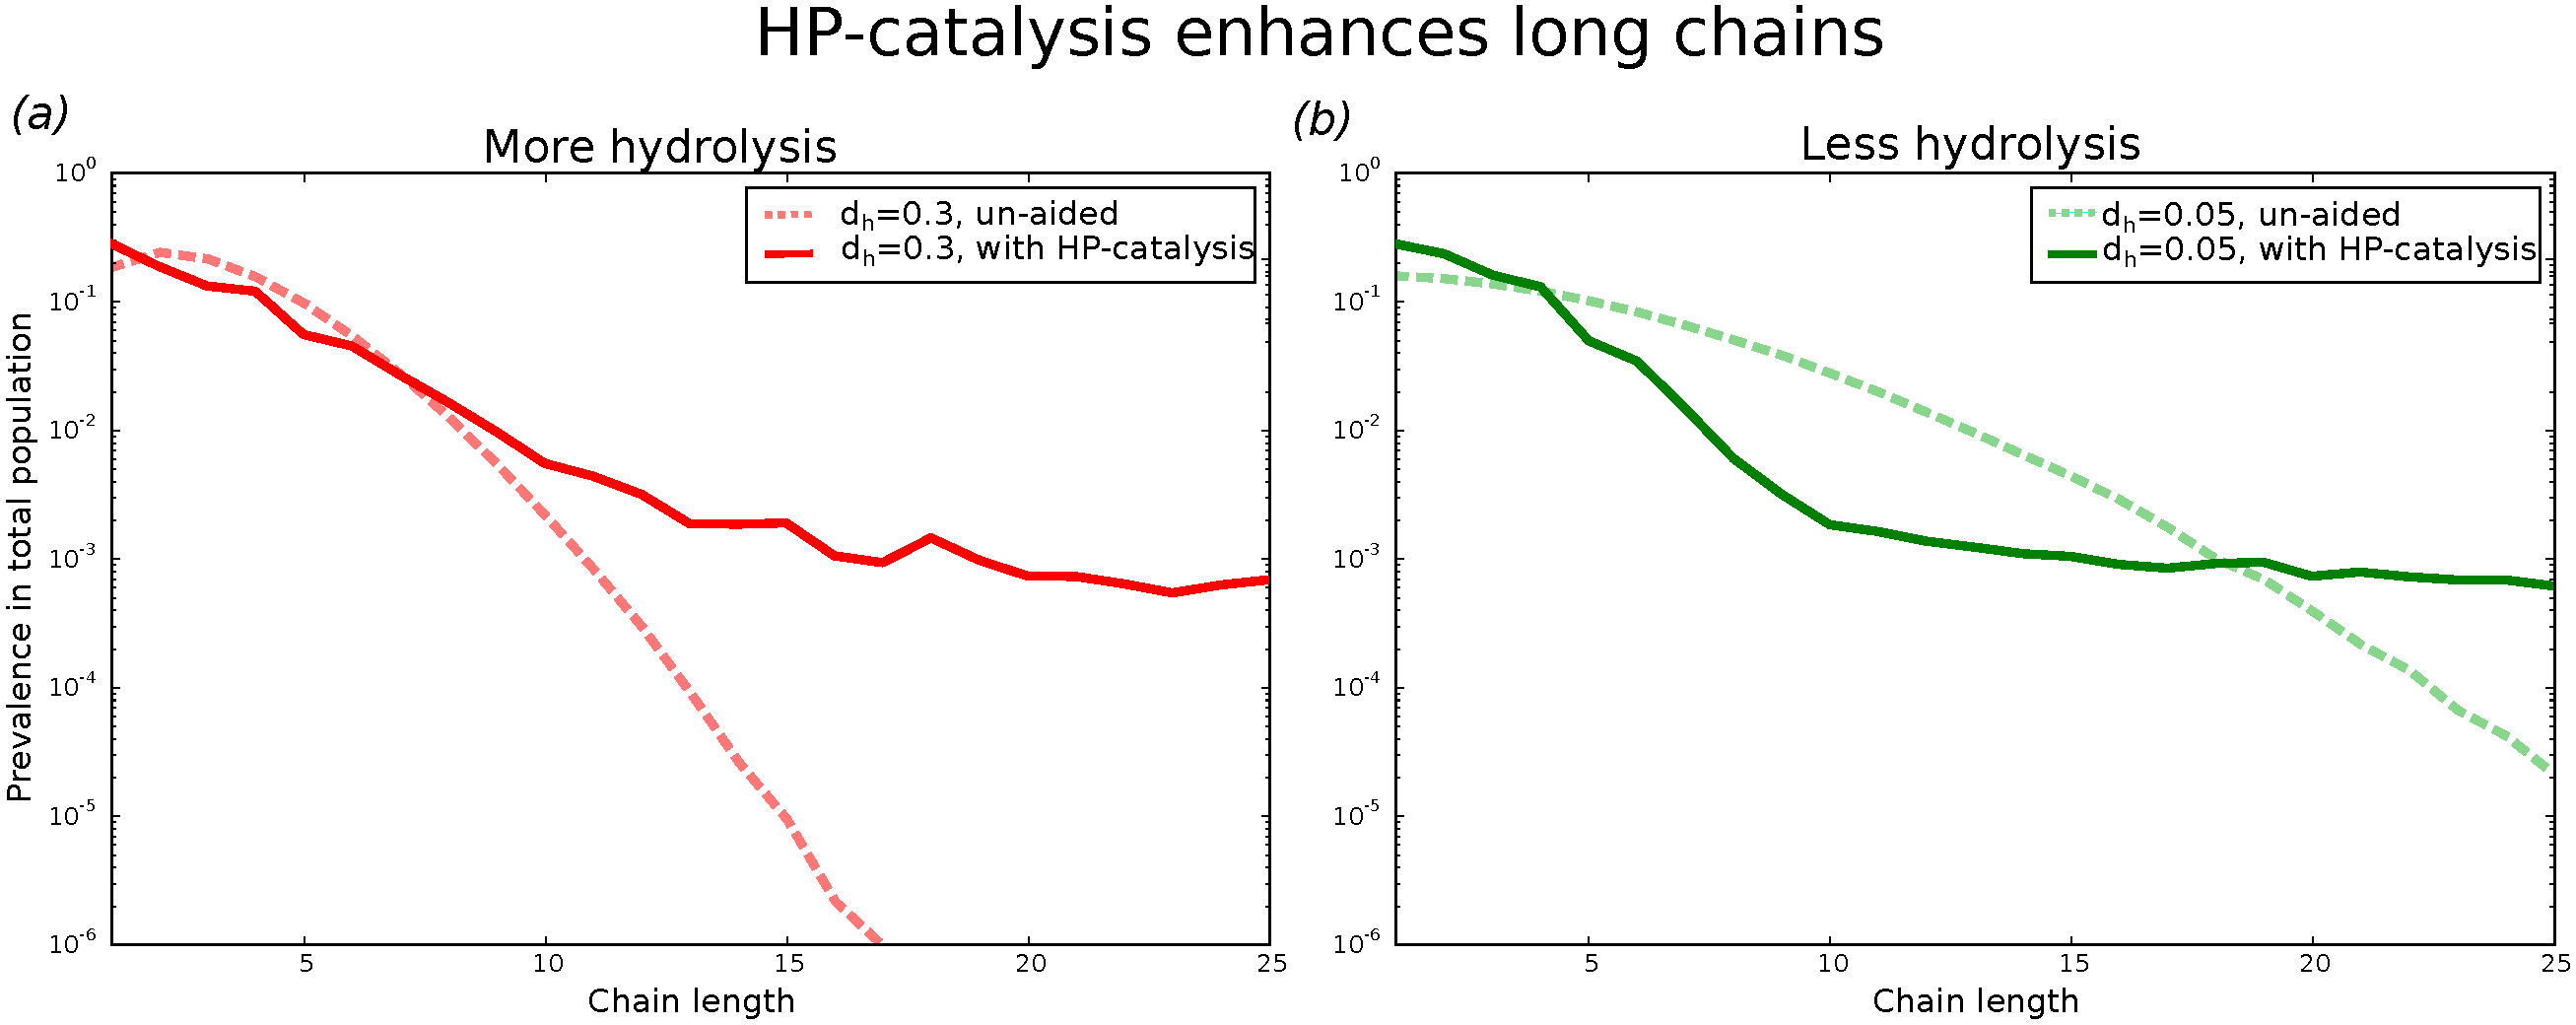
\includegraphics[width=0.95\textwidth]{pictures/flory-and-hp.pdf} 
  \caption{Dashed lines represent polymerization without folding or catalysis. Solid lines 
correspond to simulations run with folding and catalysis. For details of simulations see 
section \ref{sec:mat-sim}, Experiment 2. }
  \label{fig:sim.flory-fold}
\end{figure*}

\begin{figure}[h!]
  \centering
  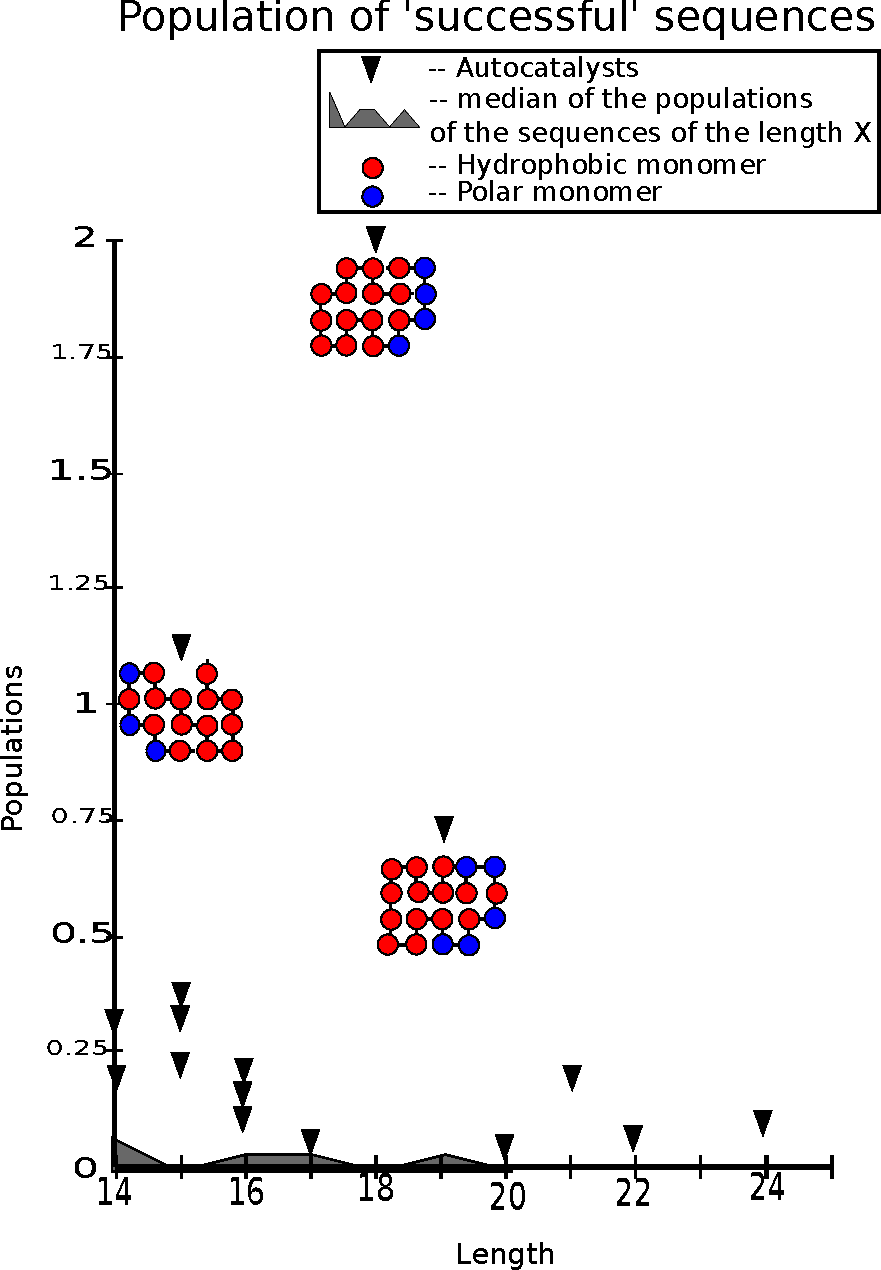
\includegraphics[width=\columnwidth]{pictures/good_seqs.pdf} 
  \caption{Some examples of dominating autocatalytic sequences. Gray lines represent regular 
non-catalytic sequence. structures on the right are native structures of autocatalytic sequences. }
  \label{fig:example1}
\end{figure}
\blue{E - We need a better fig here.  Here are 3 folded structures.  But, we are not showing 
their autocat partner.  Can we show those?  And, can we indicate how the A folds the B and how the 
B 
folds the A?}

\red{Ken -- There are no autocatalytic partners in this model. Each sequence, which can catalyze 
can be catalyzed as well. It just happen to be so. So all catalysts are auto and cross 
catalysts simultaneously. Direct interactions cannot be extracted from simulation results. There are 
some correlations of populations of sequences, but I don't understand them and cannot use.}

\blue{E -- OK, very interesting.  So, we need to say this quite specifically in the text.  
Below, I put in some possible text.  If it's correct, let's use it.  If not, let's fix it.  }

\section{Bootstrapping and autocatalysis: HP foldamers can elongate other HP chains.} 
 It has long been recognized that life's origins 
 require some form of autocatalysis~\cite{Kauffman1986,Dyson1985,Eigen1978}.  But, what mechanism 
at the molecular structural level might explain some type of molecular structural bootstrapping?  
Here, we find that a form of autocatalysis, or positive feedback, is inherent in the following 
process:  HP polymers are synthesized randomly; a small fraction of those HP polymers fold into 
relatively stable compact states; a fraction of those folded structures provide relatively stable 
`landing pad' hydrophobic surfaces; those surfaces can help to catalyze the elongation of other HP 
molecules having foldable sequences.  Figure XXX illustrates this process.
 
 \blue{E -- Can we make a series of figures showing an example of this?  
 We want specific HP sequences that fold into native structures, we then want to show their landing 
pad surfaces, and we want to show some other HP chain that then gets catalyzed on it.}
 \blue{E -- Can we say anything about what fraction of sequence space contributes?  
 I think your argument is saying that a non-trivial fraction of HP sequences are themselves 
foldamers (2\% is a number Chan and I found previously).  Etc.  It looks to me like your argument is 
saying that we have a very simple answer to a seemingly challenging question.  We don't need fancy 
explanations of auto-catalysis.  We just need to say that lots of chains can fold and create landing 
pads, and ALL of them essentially contribute to solving the Flory Problem.  Right?  Maybe we just 
need a little more detail and clarity in your paragraph below, which looks like it's making that 
point.}
 
 
In the case of hydrophobicity based interactions yet the story is different. Sequences that have 
too many $P$ residues don't fold well, and hence will be hydrolyzed rapidly.  Overly hydrophobic 
chains don't fold to unique native states as well; they are also prone to aggregation. This leaves 
only polymers with 50-80\% of hydrophobes. 
Our model supposes that only relatively unique folds are stable over long enough times to be able 
to bind and catalyze reactions.  Autocatalytic chains occupy even smaller fraction of 
sequence space due to extra requirements on structure. Yet promiscuity of the catalysis mechanism 
we employ doesn't limit them to just 1 or 2 ideal sequences, keeping their number reasonably high 
-- about 10\% of sequence space.  We found these sequences as we sought an explanation for 
the results of Figure~\ref{fig:sim.flory-fold}.  Some of the sequences and folds of these autocats 
are shown in Figure~\ref{fig:example1}.

It is also important to mention that, while we work with just binary polymers in the actual 
biological systems of, say, proteins a couple of $H$ and $P$ corresponds to 20 different amino 
acids . This means that maximum information content of the resulting HP-sequences of length $N$ is 
$\log_2(20^n)$ in fact. An evolutionary search in such an enormous space is an open-ended process 
that can lead to generating sequences with biological function. This is another advantage of 
choosing hydrophobic interaction as a leading catalytic mechanism: it unites selection with 
diversity.
%%%%%DO NOT DELETE!%%%%%%%%%%
% reviewers might ask for experiment on adaptive evolution
%%%%%%%%%%%%%%%%%%%%%%%%%%%%%

\section{Discussion}


Here are some examples of other models using autocatalytic sets
\begin{itemize}
 \item Several studies\cite{Eigen1978,Dyson1985,Kauffman1986} focused on how such self-sustaining 
systems could work if they already exist. They investigated under which conditions these systems 
indeed are self-maintaining.

\item In a more recent series of works \cite{segre1998graded,Segre2000,Markovitch2012} 
 authors numerically studied auto and cross catalysis in an artificial chemical system of 
 small mutually catalyzing  molecules. They found parameters of the system for which one can 
observe 
diversity and replication fidelity.
 Appearance of these desirable properties requires high mutual catalysis propensity.

\item In \cite{Tkachenko2014} authors studied random heteropolymers capable of template 
assisted ligation and random breakage. In such a system, they showed,  long-chained
polymers  can be sustained by the mutual catalysis of the ligation reaction. They discovered
that a system with ligation and hydrolysis is capable of first order phase transition, depending 
concentration. 
In their system the maximum length of heteropolymers is determined kinetically as a simple function 
of the ratio
between ligation and breakage rates

\item In \cite{Walker2012} authors considered a system with finite monomer source, spontaneous 
reversible polymerization
and template ligation of binary polymers. With stochastic simulations, they studied how kinetic 
rates of polymerization/degradation
affect ability of sequences to explore sequence space. Similarly to our results, the higher the 
ratio of degradation rate
over polymerization rate (in our case (hydrolysis and hydrophobic energy), the higher the diversity 
of the pool, and the lower it, the higher number of functional sequences is observed (functional 
polymers are randomly assigned). Functional sequences are able to emerge spontaneously,
they don't dominate the pool, allowing for further pool exploration. While \cite{Walker2012} and our 
system are kinetically different they experience rather similar dynamics.
\end{itemize}

Many studies focused on how in a particular situation autocatalytic systems could arise and on 
different properties of the emergent results based on type of autocatalytic mechanisms.
\begin{itemize}
\item The idea of 
autocatalysis was applied by Wu and Higgs\cite{Wu2009} to homo-polymers: while system of 
homopolymers cannot be 
complex and capable of storing information, authors showed that their system has bi-stability and 
increased proportion of long polymers.
 \item In a series of works \cite{nowak2008prevolutionary,Ohtsuki2009,Chen2012,Derr2012} 
 authors investigated binary polymers 
either capable of autocatalysis or replication. They showed that while autocatalytic system has 
bi-stability and increased ratio of longer polymers, one has to increase catalysis rate 
exponentially in order to get exponential growth of longer chains. Self-replication system on the 
other hand didn't show bi-stability, but on a positive side, relatively low replication rate 
constant brought up significant growth of longer polymers. It was also shown that self-replication 
enhances complexity of the system. The autocatalysis mechanism of this series is however very 
simple It's a self-replication performed by means of catalysis: for every reaction catalyst has to 
get attached to a growing molecule and then dissociate from it.


Significant progress has been made in attempts to make artificial autocatalytic sets in a 
laboratory\cite{VonKiedrowski1986,Lincoln2009,Vaidya2012}. These experiments, while working with 
simple artificially designed systems, exhibit a nice example of original principle.


They key difference with our work is 
that hydrophobic interaction provides a simple physical set up which produces non-linear dynamics 
with complex feedback.
This enables system to develop a non-trivial selection mechanism. Our system, as being based on 
\cite{Ohtsuki2009} model, experience bi-stability, has semi-periodic fluctuations  
and polynomial length distribution \red{??} 
\end{itemize}

\red{
\begin{itemize}
 \item Hordijk2010.
\end{itemize}
}


\subsection{2D-3D}
\begin{itemize}
 \item Folding and unfolding rates are likely underestimated in 2D case
 \item Overall length dependence is steeper in 2D case
 \item However cases are very similar and it's possible to do a mapping between them: there's a 
direct mapping between surface to volume ratio in 3D case to perimeter to area ratio in 2D case
\end{itemize}


\section{Materials and methods}\label{sec:mat}
\subsection{Simulations}\label{sec:mat-sim}
To test our hypothesis we performed direct stochastic simulations on several sets of parameters. We 
used 
\blue{PDMmod} method \cite{Bernatskiy}
% \footnote{C++ library and description can be found here: https://github.com/abernatskiy/pdmmod}. 
Stochastic simulations keep track of each 
molecular specie in the system. However simulations are limited due to computational reasons. 
First 
of all we have to explore conformational space of every polymer. This task is NP-hard (we use 
HPSandbox algorithm\cite{lau1989lattice,Dill2008} \footnote{Python implementation and description 
can be found here: http://hp-lattice.readthedocs.org/en/latest/}), so we had to limit 
maximum chain lengths to 25. We also try to keep total number of species in the low thousands, to 
avoid computational costs. We do it by introducing dilution parameter $d$: molecules are being 
removed from the system with probabilities $\propto d$. 
This either can mimic a protocell splitting and loose of materials due to it or in the case when 
system isn't bounded by any borders the fact that some molecules will diffuse away. Total number of 
molecules varies from simulation to simulation, 
however it mostly holds in the region \red{insert}.

We start our simulations with a small pool of monomers, usually below 100 molecules. 
\begin{itemize}
 \item We assume that there are enough of activated monomers in the system, so that their 
concentrations are constant. This way we don't have to track them in the simulations.

\item Polymers can therefore spontaneously grow with the rate $\ga$. Without loss of generality we 
can put this parameter equal 1; all other rates with be relative to the growth rate in this case.

\item Hydrolysis has constant rate $d_h$ per bond. Half-life time of hydrolysis bonds in neutral 
conditions and temperatures around room temperature are on the order of hundreds of 
years\footnote{Hydrolysis rate constants of oligopeptides in 
neutral conditions are of the order of $10^{-11}-10^{-10}$: $1.3  10^{-10} M^{-1}s^{-1} $ 
for benzoylglycylphenylalanine ($t_{1/2} = 128 y$)\cite{Bryant1996}, $6.3  10^{-11} M^{-1} s^{-1}$
($t_{1/2}=350 y$) for glycylglycine and $9.3 10^{-11}M^{-1} s^{-1}$ for glycylvaline
\cite{Smith1998}.}. We test hydrolysis rate constants to be about $0.001-1$ of polymerization rate 
constants. This way we account for polymerization conditions, which happens on the order of days 
to years.

\item We also import monomers into system with rate $a\gg1$. It is safe to assume that we would 
have enough monomers in the system and import of monomers wouldn't be a bottleneck of reactions 
chain. Therefore we explore big values of $a\propto 
10^2,10^3\ga$

\item Dilution parameter $d$ mimics cell division and loss of the matter because of that. From 
\ref{sec:nowak-steady} we see that total mass of the system is  $ M\propto\frac{a}{\ga}, \qquad 
d\approx \ga\quad \mbox{or}\quad d\gg \ga$ and $M\propto \frac{a}{\ga}\frac{d}{2\ga} ,\qquad 
d\ll\ga$. Therefore we explore valued of $d$ from $\propto 0.01\ga$ to $\propto 1\ga$. Given 
values of $a$ we'll explore various populations from $\propto 10^2$ to $\propto 10^5$ monomers per 
cell.

\item (\red{Fix this after discussion}) Folding and unfolding reactions happen very quickly with 
the unfolding rate constants of 
$k_{unf}\gg\ga$ and folding rate constant of $k_{unf}\cdot\exp(E_{native}/kT)$.

$E_h$ in our experiments is around $1-2$kT\red{\cite{?}}. $k_{unf}$ we keep $\propto 10^2$, which 
gives us range of unfolding rates from a reaction per hours and days and range of folding rates 
from a reaction per hours to fractions of a second.

\item Catalysis rate is proportional to the exponent of hydrophobic energy $E_h$ and number of 
contacting hydrophobes $n_c$: $\ga\cdot\exp(E_{h}\cdot n_{c}/kT)$. Number of hydrophobic contacts 
for the short HP-sequences is about $3-6$. With the hydrophobic energies of $1-2$kT this gives us 
catalysis rates around hours and days for one reaction.

% \item Some experiments also include aggregation reactions for the long hydrophobic chains.
\end{itemize}
We looked at the lengths distribution in steady state. In order to account for stochastic effects 
we took average over several realizations. We also looked at the time evolutions of specific 
chains to investigate correlations between sequences and internal dynamics. The simulations were 
performed on Computing Cluster of Laufer Center. See \blue{appendix} for simulation details.
\begin{center}
\begin{table*}[h]
\begin{tabular}{| p{3.5cm} | l | p{3cm}| p{3.4cm}| p{3.4cm} |}
\hline
Constant name & Symbol  & Normalized simulation value & Simulation 
value (deduced) per $1M$& Value from literature, per $1M$\\
\hline
Polymerization rate constant & $\ga$ &  1 & $\propto 1\,month^{-1}$ & ??\\
\hline
Hydrolysis  rate constant & $d_h$ & $\propto 10^{-1}\textendash10^{-4}$ & $\propto 1\,month^{-1}-- 
10^{-3}year^{-1}$ & $\propto 10^{-3}year^{-1}$ 
\cite{Bryant1996,Smith1998,Danger2012}\\
\hline
Dilution rate constant & $d$&$\propto 10^{-2}-1$ & $\propto 0.1year^{-1} -- 
10^{-3}year^{-1}$ & \begin{center}\textemdash \end{center}
 Is\,used\,to\,keep model from 
overflowing \\
\hline
Monomer import rate constant & $a$ & $\propto 10^2-10^3$  & $\propto 1 - 10^2 day^{-1}$ & ??\\
\hline
Number of rotational freedoms& $z$ & $1.5-2.5$  & $1.5-2.5$ & 
??\\
\hline 
Hydrophobic energy per $kT$ & $e_h$ & $1-2$ & $1-2$ & $0-3.3$ \cite{Wimley1996}
\\ \hline
\end{tabular}
\caption{Parameters of our simulations: we set polymerization rate constant to 1. All other rate 
constants were 
measured in terms of it. However mapping one of the constants to lab/prebiotic values fixes the 
rest of the rate 
constants. We compare them with the ones found in the origins of life literature.}
\label{tab:methods}
\end{table*}
\end{center}

\paragraph{Experiment 1. Reproduction of Flory distribution.}\label{sec:expt1}
We started simulations with small pool of monomers (20 H and 20 P). We ran 30 identical  
simulations for 200 s each, with measurements taken every 0.1s. Steady state is being achieved 
around 30-50s. To calculate length distribution, we took one trajectory and calculated average 
over time over all time points after 100s; so we got 1000 time points for every chain length, over 
which we averaged. The rate of conversion of activated monomers into regular ones is $a=100$. We 
took dilution rate of $d=0.5$. We ran experiments for 2 hydrolysis rates: $d_h=0.3$ and $d_h=0.03$.
We varied hydrolysis and dilution rates. Experiments with $d_h=0$ reproduce accurate exponential 
curves; adding hydrolysis, however, slows down distribution around short lengths. This effect is 
due to constant concentration of activated monomers: there's no competition for ``food''. This 
enriches population of short chains, however doesn't affect longer chains significantly, leaving 
their distribution nearly exponential.

\paragraph{Experiment 2. Introduction of HP-folding}



\paragraph{Experiment 3. Introduction of HP-catalysis.}
\textbf{\red{Set of parameters. Do not delete so far.} }\\
Experiment ``test-dhd''. Simulations \# 07-13
\begin{enumerate}
 \item 'aggregation = 100.0',
 \item  'importH = 200.0',
\item   'eH = 2.0',
\item   'importP = 200.0',
  \item 'growth = 1.0',
  \item 'maxLength = 25',
  \item 'aggrAt = 1.0',
\item 'z = 1.2',
  \item 'degradation = 0.3',
  \item hydrolysis = 0.001 0.003 0.005 0.01 0.03 0.05 0.1
\end{enumerate}
Simulations with degradation = 0.1 are also very interesting


In addition to folding in this \textit{in-silico} experiment we introduced interaction between 
proteins. All parameters are as above. We varied parameters of the simulations, and noticed 
significant stability of the length distribution towards change of $d_h$ and $d$. distribution is 
sensitive towards hydrophobic energy, as expected. Chain length distribution has a noticeably 
non-exponential behavior in the region when $E_h= 1-3 kT$



 \newpage
\appendix
\section{HP catalysis}
\begin{figure}[h!]
  \centering
  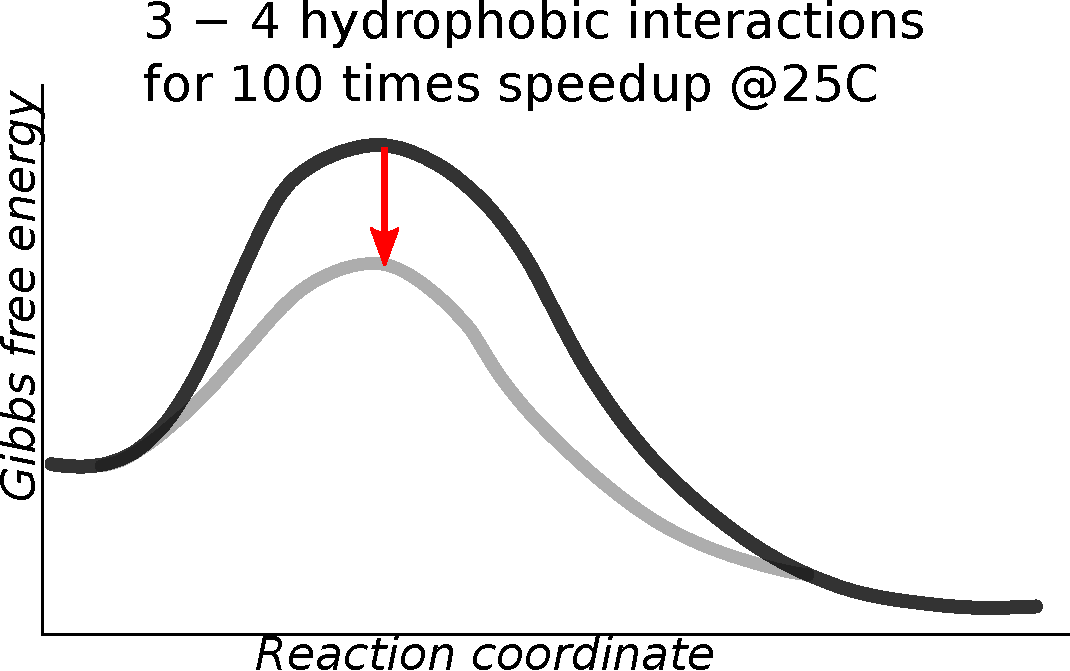
\includegraphics[width=0.9\columnwidth]{pictures/hp-catalysis-b.pdf} 
  \caption{Catalyst catalyzes a growing of an unfolded hp-polymer. 
           Having just 3-4 hydrophobic contacts is enough to lower an 
           activation barrier for $\propto 100$ times at room 
           temperature.}
  \label{fig:hp-catalysis-b}
\end{figure}


\begin{figure}[h!]
  \centering
  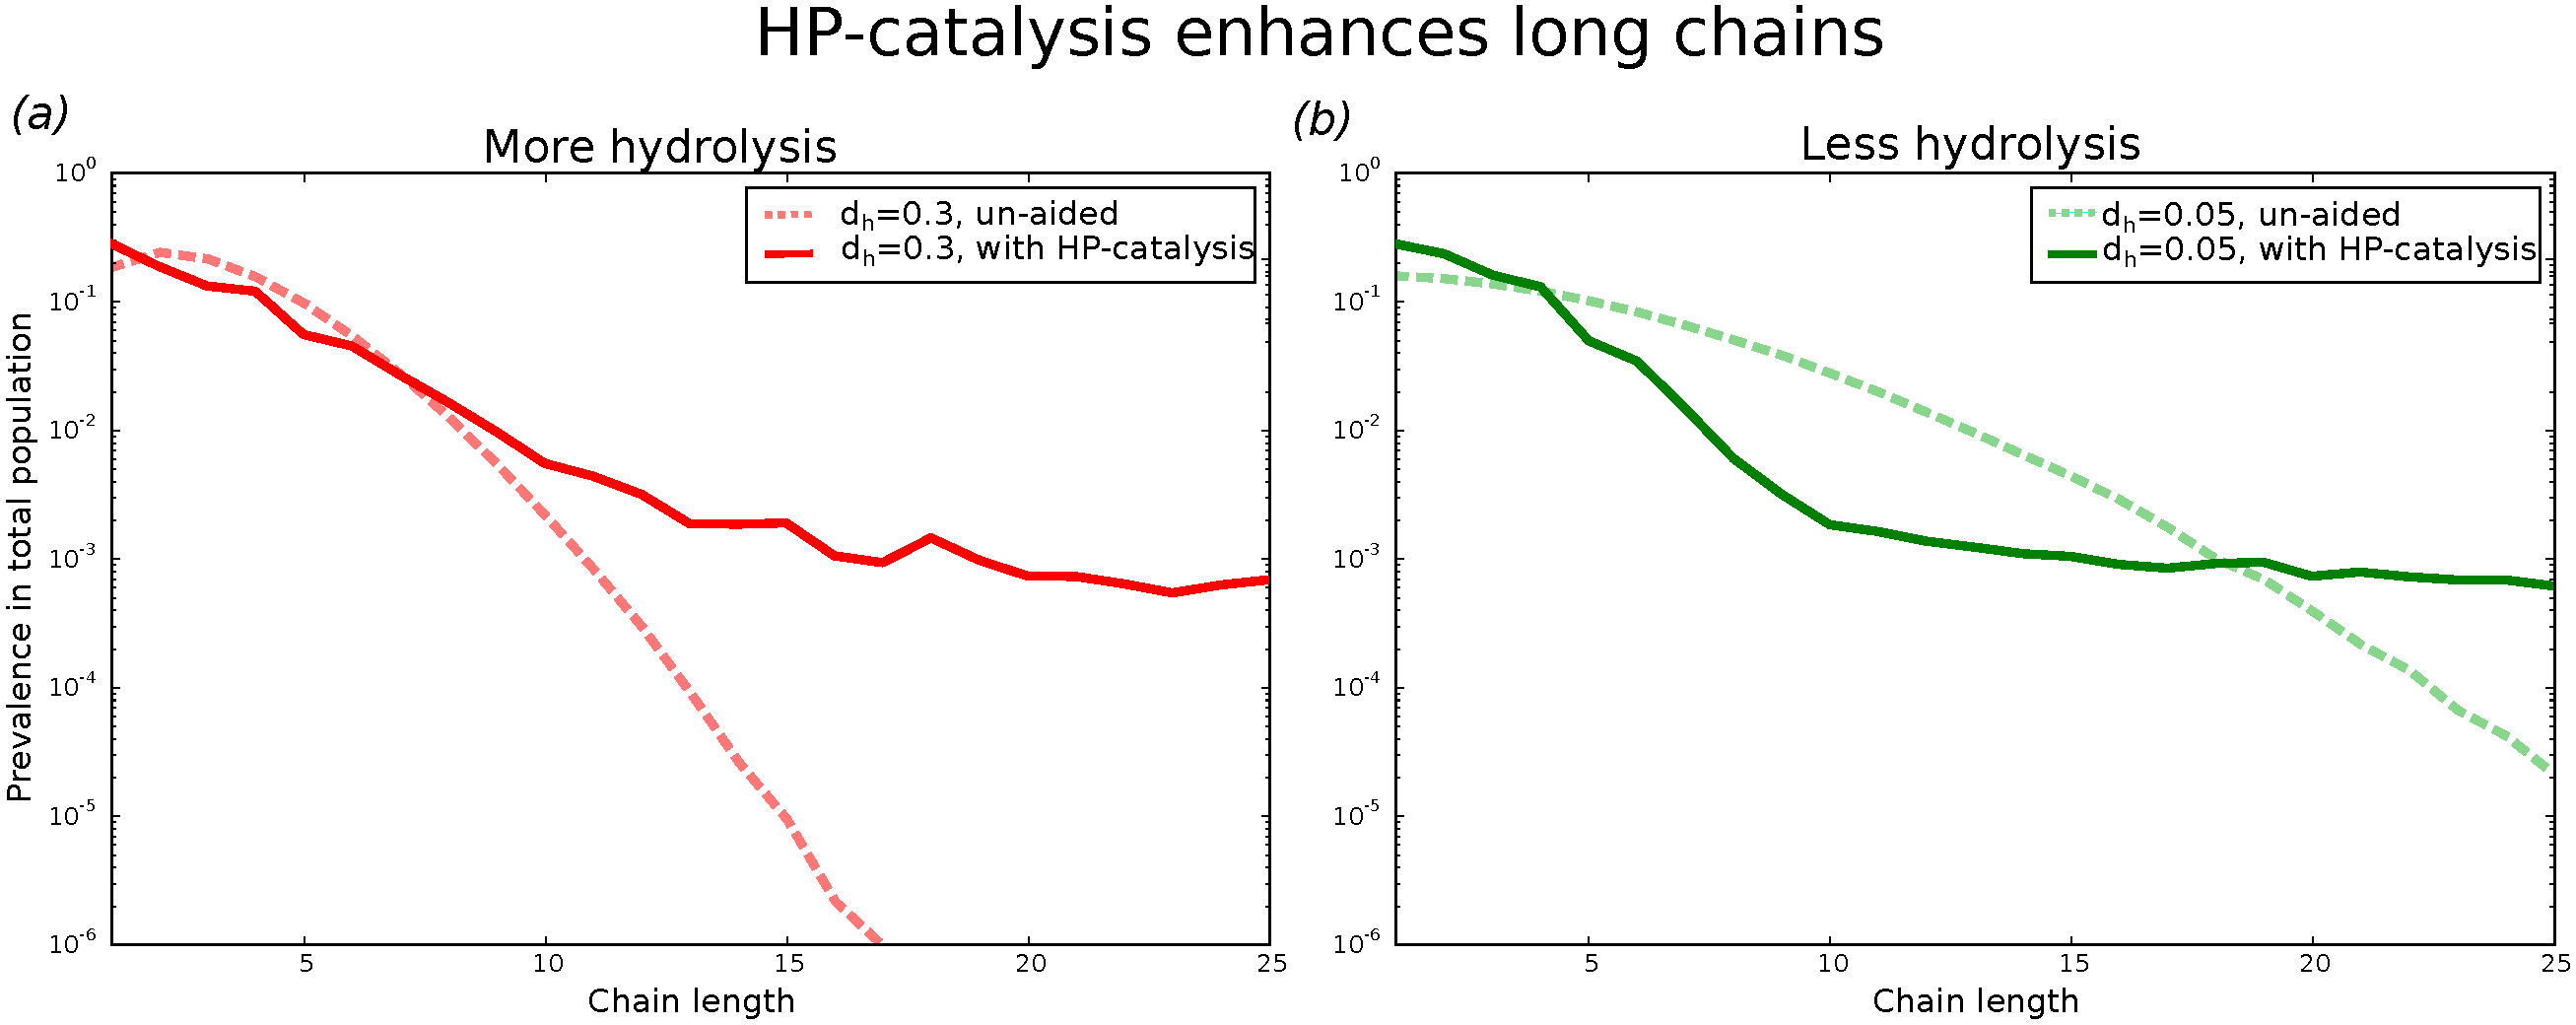
\includegraphics[width=\columnwidth]{pictures/flory-and-hp.pdf} 
  \caption{}
  \label{fig:flory-and-hp}
\end{figure}

\section{Details of the kinetic model.}
\red{\textbf{Change}}

% We describe here briefly the Nowak model \cite{nowak2008prevolutionary,Ohtsuki2009,Chen2012}
% 
% \blue{E - Is ours different than Nowak's?  If so, spell out how it's different.}
% 
% We enumerate all the polymers, so that $x_i$ is population of $i^{th}$ monomer, and $x_{i'}$ is a 
% population of its precursor.
% 
% Equations are:
%   \begin{eqnarray}
%    \mbox{One mers:}&& \dot{x_i}=a-2\ga x_i-dx_i \\
%      \mbox{2+ mers:}&& \dot{x_i}=\ga x_{i'}-(2\ga+d)x_i
%   \end{eqnarray}
% 
% Now, we consider the dynamics of the steady state, $\dot{x_i}=0$
%   \begin{eqnarray}
%    \mbox{One mers:}&& 0=a-2\ga x_i-dx_i \\
%      \mbox{2+ mers:}&& 0=\ga x_{i'}-(2\ga+d)x_i
%   \end{eqnarray}
%   So we have:
%    \begin{eqnarray}
%    \mbox{One mers:}&& x_i=\frac{a}{2\ga+d} \\
%      \mbox{2+ mers:}&& x_i=\frac{\ga}{2\ga+d}x_{i'}
%   \end{eqnarray}   
%  Therefore for every sequence of length $l$ we get:
%    \begin{equation}
%    \boxed{ x_l=\frac{a}{\ga}\pt{\frac{\ga}{2\ga+d}}^l}
%    \end{equation} 
% 
% Population of all the sequence of length $l$ is therefore:
%   \begin{equation}
%     p_l=\frac{a}{\ga}\pt{\frac{\ga}{2\ga+d}}^l2^l=\frac{a}{\ga}\pt{\frac{2\ga}{2\ga+d}}^l=
%     \frac{a}{\ga}\pt{\frac{1}{1+d/2\ga}}^l
%   \end{equation} 
% If we denote $x\equiv\frac{d}{2\ga}$, population of all the sequences of length $l$ will be:
% \begin{equation}
% \boxed{ p_l=\frac{a}{\ga}\pt{\frac{1}{1+x}}^l}
% \end{equation} 
% Total mass of all the sequences is:
% \begin{equation}
%  M=\sum_{l=0}^{\infty}lp_l
% \end{equation} 
% \begin{equation}
%  M=\sum_{l=0}^{\infty}\frac{a}{\ga}l\pt{\frac{1}{1+x}}^l
% \end{equation} 
% According to \cite{Gradstein1980} the sum will be
% \begin{equation}
%  M=\frac{a}{\ga}\frac{\frac{1}{1+x}}{\pt{1-\frac{1}{1+x}}^2}=\frac{a}{\ga}\pt{\frac{1+x}{x}}
% \end{equation}
% Therefore total mass is:
%   \begin{equation}
%    M=\frac{a}{\ga}\pt{1+\frac{1}{x}}
%   \end{equation} 
% Remember that $x=d/2\ga$. It means that values of $d$ $d\approx \ga$ or $d\gg \ga$ produce total 
% masses 
% \begin{equation}
%  M\propto\frac{a}{\ga}, \qquad d\approx \ga\quad \mbox{or}\quad d\gg \ga
% \end{equation} 
% while very small values of $d:\,d\ll\ga$ produce total masses 
% \begin{equation}
% M\propto \frac{a}{\ga}\frac{d}{2\ga} ,\qquad d\ll\ga
% \end{equation}



 \bibliography{library}
\bibliographystyle{achemso}

\end{document}

%%% Local Variables:
%%% mode: latex
%%% TeX-master: t
%%% End:

%  LocalWords:  prebiotic prebiotically nucleotides polypeptides mers
%  LocalWords:  enzymatically oligomers clays asymptote biopolymers
%  LocalWords:  peptides et al montmorillonite hectorite Gly unf dx
%  LocalWords:  oligouridylates phosphoimidazolide lp
